Newspaper archives are fundamental resources for historians, librarians, and social scientists \cite{Chassanoff,allen} because they offer a detailed primary source record of how social processes evolve across time \cite{pierson2004politics}.
For instance, social researchers have used news archives to examine vital questions such as why the United States abolished slavery \cite{foner1995free} and how different jurisdictions slowed the spread of the 1918 flu \cite{jama}.
While historians are known to use archives in different ways (e.g., sequential browsing \cite{allen}), prior work reports that historians often look for ``specific keywords'' \cite[p. 2]{allen} in newspaper corpora.
For instance, scholars in history and social science journals describe tracking down and reviewing occurrences of words like
``William Benbow'' \cite{Putnam},
{``Frances Maule''} \cite{FrancesMaule},
{``watermelon'' }\cite{watermelon},
{``Japanese beetles''} \cite{japanesebeetles},
{``refugee''} \cite{katrinarefugee},
{``Loving''} \cite{Loving}, and
{``race suicide''} \cite{racesuicide}
in news archives
to help answer questions about society.
In this work, we describe such search terms (e.g., ``William Benbow'') as \textbf{queries} and we describe each exact occurrence of a query in an archive as a query \textbf{mention}.
(Section \ref{s:limits_and_future} discusses possible improvements to exact string matching.)
We then describe the task of locating query mentions as \textbf{mention gathering}, and the closely-related task of reviewing and drawing conclusions from query mentions within the context of surrounding text as \textbf{mention analysis}.\footnote{
Using terminology from prior work \cite{pirolli2005sensemaking}, it is possible to interpret mention gathering as a kind of information foraging and mention analysis as a kind of sensemaking.}
We formally define these terms and tasks in Section \ref{s:needs_formal_problem}.

Much prior work in interactive text analytics (Section \ref{s:related}) does not focus on helping people investigate mentions of a query word in context.
Instead, prior systems (designed for different use cases) focus on the analysis of other latent and observable textual units, such as topics \cite{tiara}, events \cite{eventriver}, document metadata \cite{pivotpaths}, clusters \cite{starspire}, interrelated entities \cite{Gorg2013JigsawReflections}, or thematic hierarchies \cite{overview}. Using terminology from Chuang et al.\ \cite{chuangheer}, who articulate best practices for text analytics, because such systems do not use query words in context as their central ``unit of analysis,'' they offer ``visual encodings,'' ``modeling decisions,'' and interactions which are are poorly ``aligned'' to the ``tasks, expectations, and background knowledge'' of historians and archivists. 

This misalignment means that prior text analytics systems have concrete downsides for mention gathering and analysis. For example, some prior systems focused on helping people analyze high-level text units such as temporal trends in word use (e.g., ThemeRiver \cite{ThemeRiver}) do not show query words in underlying text. Similarly, other systems offer only indirect and incomplete access to query words in context, via extraneous mediating abstractions. We detail these limitations in Section \ref{s:related_comparison}.


\begin{figure}[t!]
\centering
\frame{\includegraphics[width=1.0\textwidth]{figures/system.pdf}}
\caption[The \ours~interface]{
\ours, an interactive text analytics system for helping historians investigate queries in news archives.
Features (letters A to K) include: (D) a Time Series View showing the frequency of a user's query through time, (H) a linked Document Feed showing a skimmable query-oriented summary of every mention of the query in the corpus, and (I) a linked Document Viewer showing a selected news story, with text from the query-oriented summary highlighted in yellow. 
Section \ref{s:system} describes the full system, explaining each feature.\vspace{.05cm}
}
\label{f:system_cc}
\end{figure}



However, in practice, social researchers such as Shinozuka \cite{japanesebeetles} and others \cite{Putnam, FrancesMaule, Loving, watermelon, katrinarefugee, racesuicide} do not report using specialized text analytics systems.
Instead, these experts describe using traditional {\Baselongname~engines} like ProQuest \cite{proquest} to analyze query words in corpora. 
(We use \textit{corpus} and \textit{archive} interchangeably; we assume the corpus is an archive.)
Traditional \Baselongname~tools return relevance-ranked document lists in response to a free-text query.
Because they are widely used in historical practice \cite{allen, Putnam, Chassanoff, FrancesMaule},
we propose they are baselines for mention gathering and analysis (Section \ref{s:baseline}). 

Yet \Baselongname~tools also have limitations for finding and analyzing query words in context.
First, because almost all words are very rare (a well-known property of text \cite{Zipf49}), any given query will very likely appear only a small number of times within a document.
This means that people reviewing a ranked document list will have to examine many passages within documents that do not directly mention their query term.
While search within document features (e.g.\ \texttt{control + F} in Chrome \cite{chromeF}) can certainly help, gathering and analyzing query words in context using a \Baselongname~system still requires opening each article in its own window or tab,\footnote{Showing a single document in a single window or tab is a common interface pattern. It is employed, for instance, in the Overview \cite{overview} and Jigsaw \cite{ubigsaw} document viewers, and in traditional search user interfaces, which often link to individual documents from a main search engine results page \cite[Section 6.3]{croft2010search}.} locating mentions within the article, reading passages which mention the query, and integrating information from such passages with existing knowledge, before moving on to the next document in the corpus.
This means that people must context switch across stories as they perform a multi-step process to gather and analyze query mentions in context, keeping track of information from one document as they jump to the next (see Figure \ref{f:field_study_loop}).
Navigating between documents is thought to impose cognitive costs in \Baselongname~tools \cite{orientationWhite,fluidLinks}, and context switching across views is thought to impose cognitive costs in visual analytics systems \cite{Baldonado}.

{
\begin{table}[t!]
\centering
% \small %uncomment_for_thesis 
\begin{tabular}{@{}l | cc@{}} \toprule
                       User study   & {Num. participants} & {Total hours} \\ \hline
Needfinding study to guide system design (Sec.\ \ref{s:needs})  & 5                             & 4.5                  \\ % \cline{1-4}
Expert interview study to evaluate \ours~features (Sec.\ \ref{s:usabilitystudy}) & 5                             & 5                    \\ 
Field study to test \ours~in the wild (Sec.\ \ref{s:fieldstudy}) & 2                             & 5    \\                
Quantitative comparison study~(Sec.\ \ref{s:crowdstudy}) &             \totalN                 & \totalNmin    \\ \bottomrule                 
\end{tabular}
\caption[A summary of three separate user studies with expert historians and archivists]{This work presents four separate user studies with historians and archivists. Section \ref{s:needs} describes institutional approval. Tables in the Appendix describe the backgrounds of participants in greater detail.}\label{t:all_user_studies}
\end{table}
}

Noting the importance of historical investigation and the limitations of existing tools (for mention gathering and analysis), we propose the \ours\footnote{Clio is a common prefix (e.g., ClioVis \cite{ClioVis}), implying a connection with history.}~text analytics system, to help historians in their work investigating query words in an archive.
Unlike prior tools, which focus on the analysis of other textual units like topics or hierarchies (Section \ref{s:related_comparison}), \ours~is designed and built to help people analyze query words in context, reflecting the needs and practices of historians and archivists.
Creating tools around the ``tasks, expectations and background knowledge" of end users is believed to be a best practice in text analytics \cite{chuangheer}.

We both worked with and studied historians and archivists to prototype \ours.
This process revealed intertwined technical and design requirements for our system (Section \ref{s:needs}).
First, working with historians revealed the importance of comprehensive review in historical research (Section \ref{s:needs_comprehensive}). 
Thus, \ours~includes a novel Document Feed feature, which uses natural language processing (NLP) techniques to show a comprehensive query-focused summary of every single mention of a user's query term across a corpus.
Similarly, because we found that historians require transparency and contextual information to interpret evidence, \ours's~novel Document Feed is presented alongside a more traditional linked full-text Document Viewer, which is designed to quickly and transparently show text from the summary within the context of full-length documents.
Finally, because because temporal analysis is crucial to historians, \ours~also includes an interactive Time Series View to provide an overview of a query through time.
Together, through these and other features (Section \ref{s:system}), \ours~offers a text analytics system organized around the analysis of query mentions in context. 

In total, our work offers the following:
\begin{itemize}
\item \textbf{A synthesis of extensive prior research in text analytics} (Section \ref{s:related}). 
In reviewing prior work on interactive analysis of text across time, we found that many efforts from the NLP, HCI, and Visualization communities focus on offering overviews of corpus contents.
Such overviews might help users formulate queries, but are not designed for the query-oriented tasks of mention gathering and analysis (when the user already knows what to search for).
\item \textbf{An investigation into user needs and requirements} (Section \ref{s:needs}). 
To build our tool, we translated prior research on historians' information-seeking behavior into concrete guidelines for system design. 
We also validated and contextualized prior work by conducting five needfinding interviews with historians and archivists, while gathering feedback on early prototypes.
This process revealed a need for transparency, trustworthiness, context, and comprehensiveness in archival tools, which might 
inform future work on historical search \cite{histdiv,expedition} and text summarization \cite{das2007survey,nenkova2012survey}.
\item \textbf{The \ours~system} (Section \ref{s:system}). \ours~is an open-source, text analytics system designed to help historians find and analyze query mentions in context. The system~combines novel query-focused summarization methods with more traditional features like linked views, in-text highlighting, and time series plots to help experts quickly, comprehensively, and transparently find and review query mentions across an archive. Code for the system is available on GitHub: \texttt{https://github.com/AbeHandler/ClioQuery}.
\item \textbf{An evaluation of specific \ours~features} (Sections \ref{s:usabilitystudy} and \ref{s:qualresults}). 
To test the utility and usability of \ours, we conducted an expert interview study with five social researchers, who used the system to answer a historical question from news archives.
After methodically coding qualitative feedback, we learned that many experts found \ours's skimmable, query-focused summaries useful because they condensed documents to facilitate quick review of query mentions.
We also learned that linking summary text with underlying source documents using in-text highlighting was essential because it offered necessary context for interpreting summary output.
\item \textbf{An evaluation of \ours~in the wild} (Section \ref{s:fieldstudy}). To test \ours~in a realistic setting, we deployed the system in a field study with two historians, who used \ours~to answer questions from their own research.
In comparing experiences with \ours~to prior experiences with \Baselongname~systems, one historian explained how \ours~reduced their reading burden, and another explained how text summarization features facilitated rapid mention gathering and analysis.
\item \textbf{A quantitative comparison with \Baselongname~tools} (Section \ref{s:crowdstudy}). We conducted a quantitative crowd study to directly compare \ours~with baseline \Baselongname~search systems. In the study, we observed that participants who used \ours~to complete a reading comprehension task modeled on a real historical research question correctly answered significantly more reading comprehension questions than participants who completed the same task using a \Baselongname~system.
\end{itemize}

\noindent We conclude by discussing our findings (Section \ref{s:discussion}), reviewing limitations and future work (Section \ref{s:limits_and_future}), and describing possible applications of features and ideas from \ours~in other query-oriented settings, beyond historical research (Section \ref{s:conclusion_cc}).


\begin{figure}[!ht]
\begin{subfigure}{1\textwidth}
  \centering
  % include second image
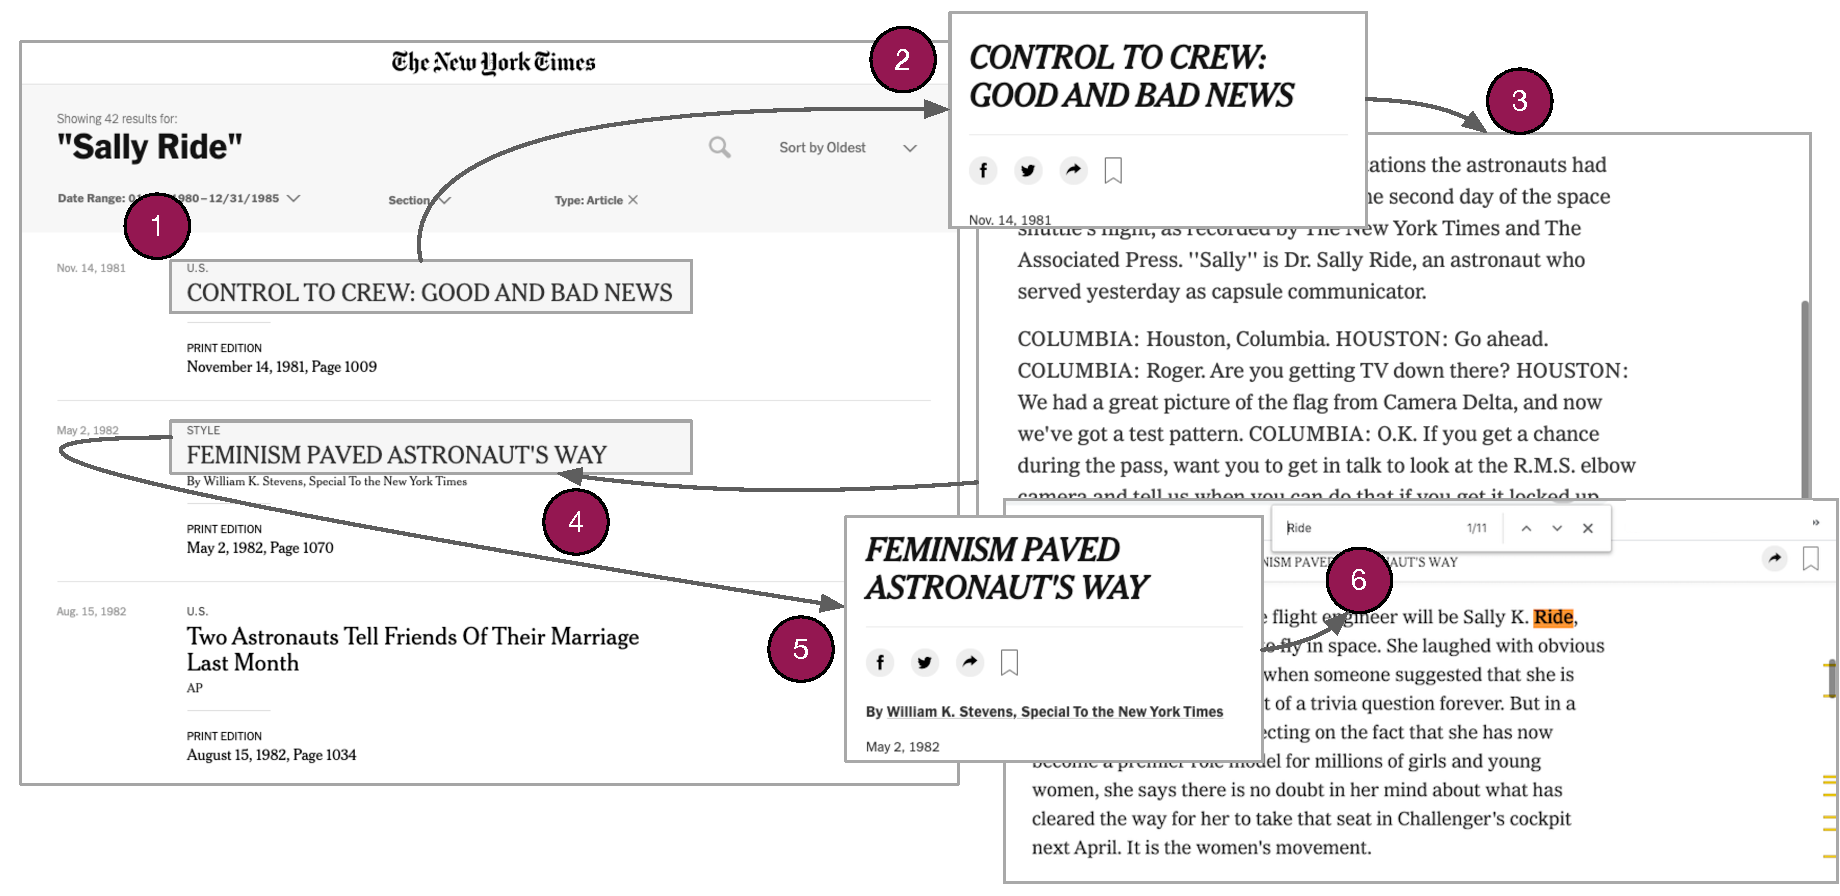
\includegraphics[width=.71\linewidth]{figures/workflow_fig/open_locate_loop_nyt.pdf}
  \subcaption{
% \footnotesize %  uncomment for thesis
  A user investigates Sally Ride by performing {\burdensome~and analysis} using the \textit{New York Times} web archive \cite{nytwebsite}, a baseline keyword document search interface (Section \ref{s:baseline}). They first (1) click the top headline on the search engine results page (left) in order to (2) {open} a document in a new tab (shown on the right) and then (3) scroll down to {locate} mentions of ``Ride'' in the linked news story. The user {reads} and analyzes these mentions and then (4) context switches to the second document by clicking the second headline on the results page. This (5) opens a new story in a new tab. For this second document, they (6) use a search in document feature \cite{chromeF} (i.e.\ \texttt{Control+F}) to help {locate} mentions of ``Ride'' within the story.
}\label{f:field_study_1} \vspace{.25cm}
\end{subfigure}
\begin{subfigure}{1\textwidth}
  \centering
  % include first image
  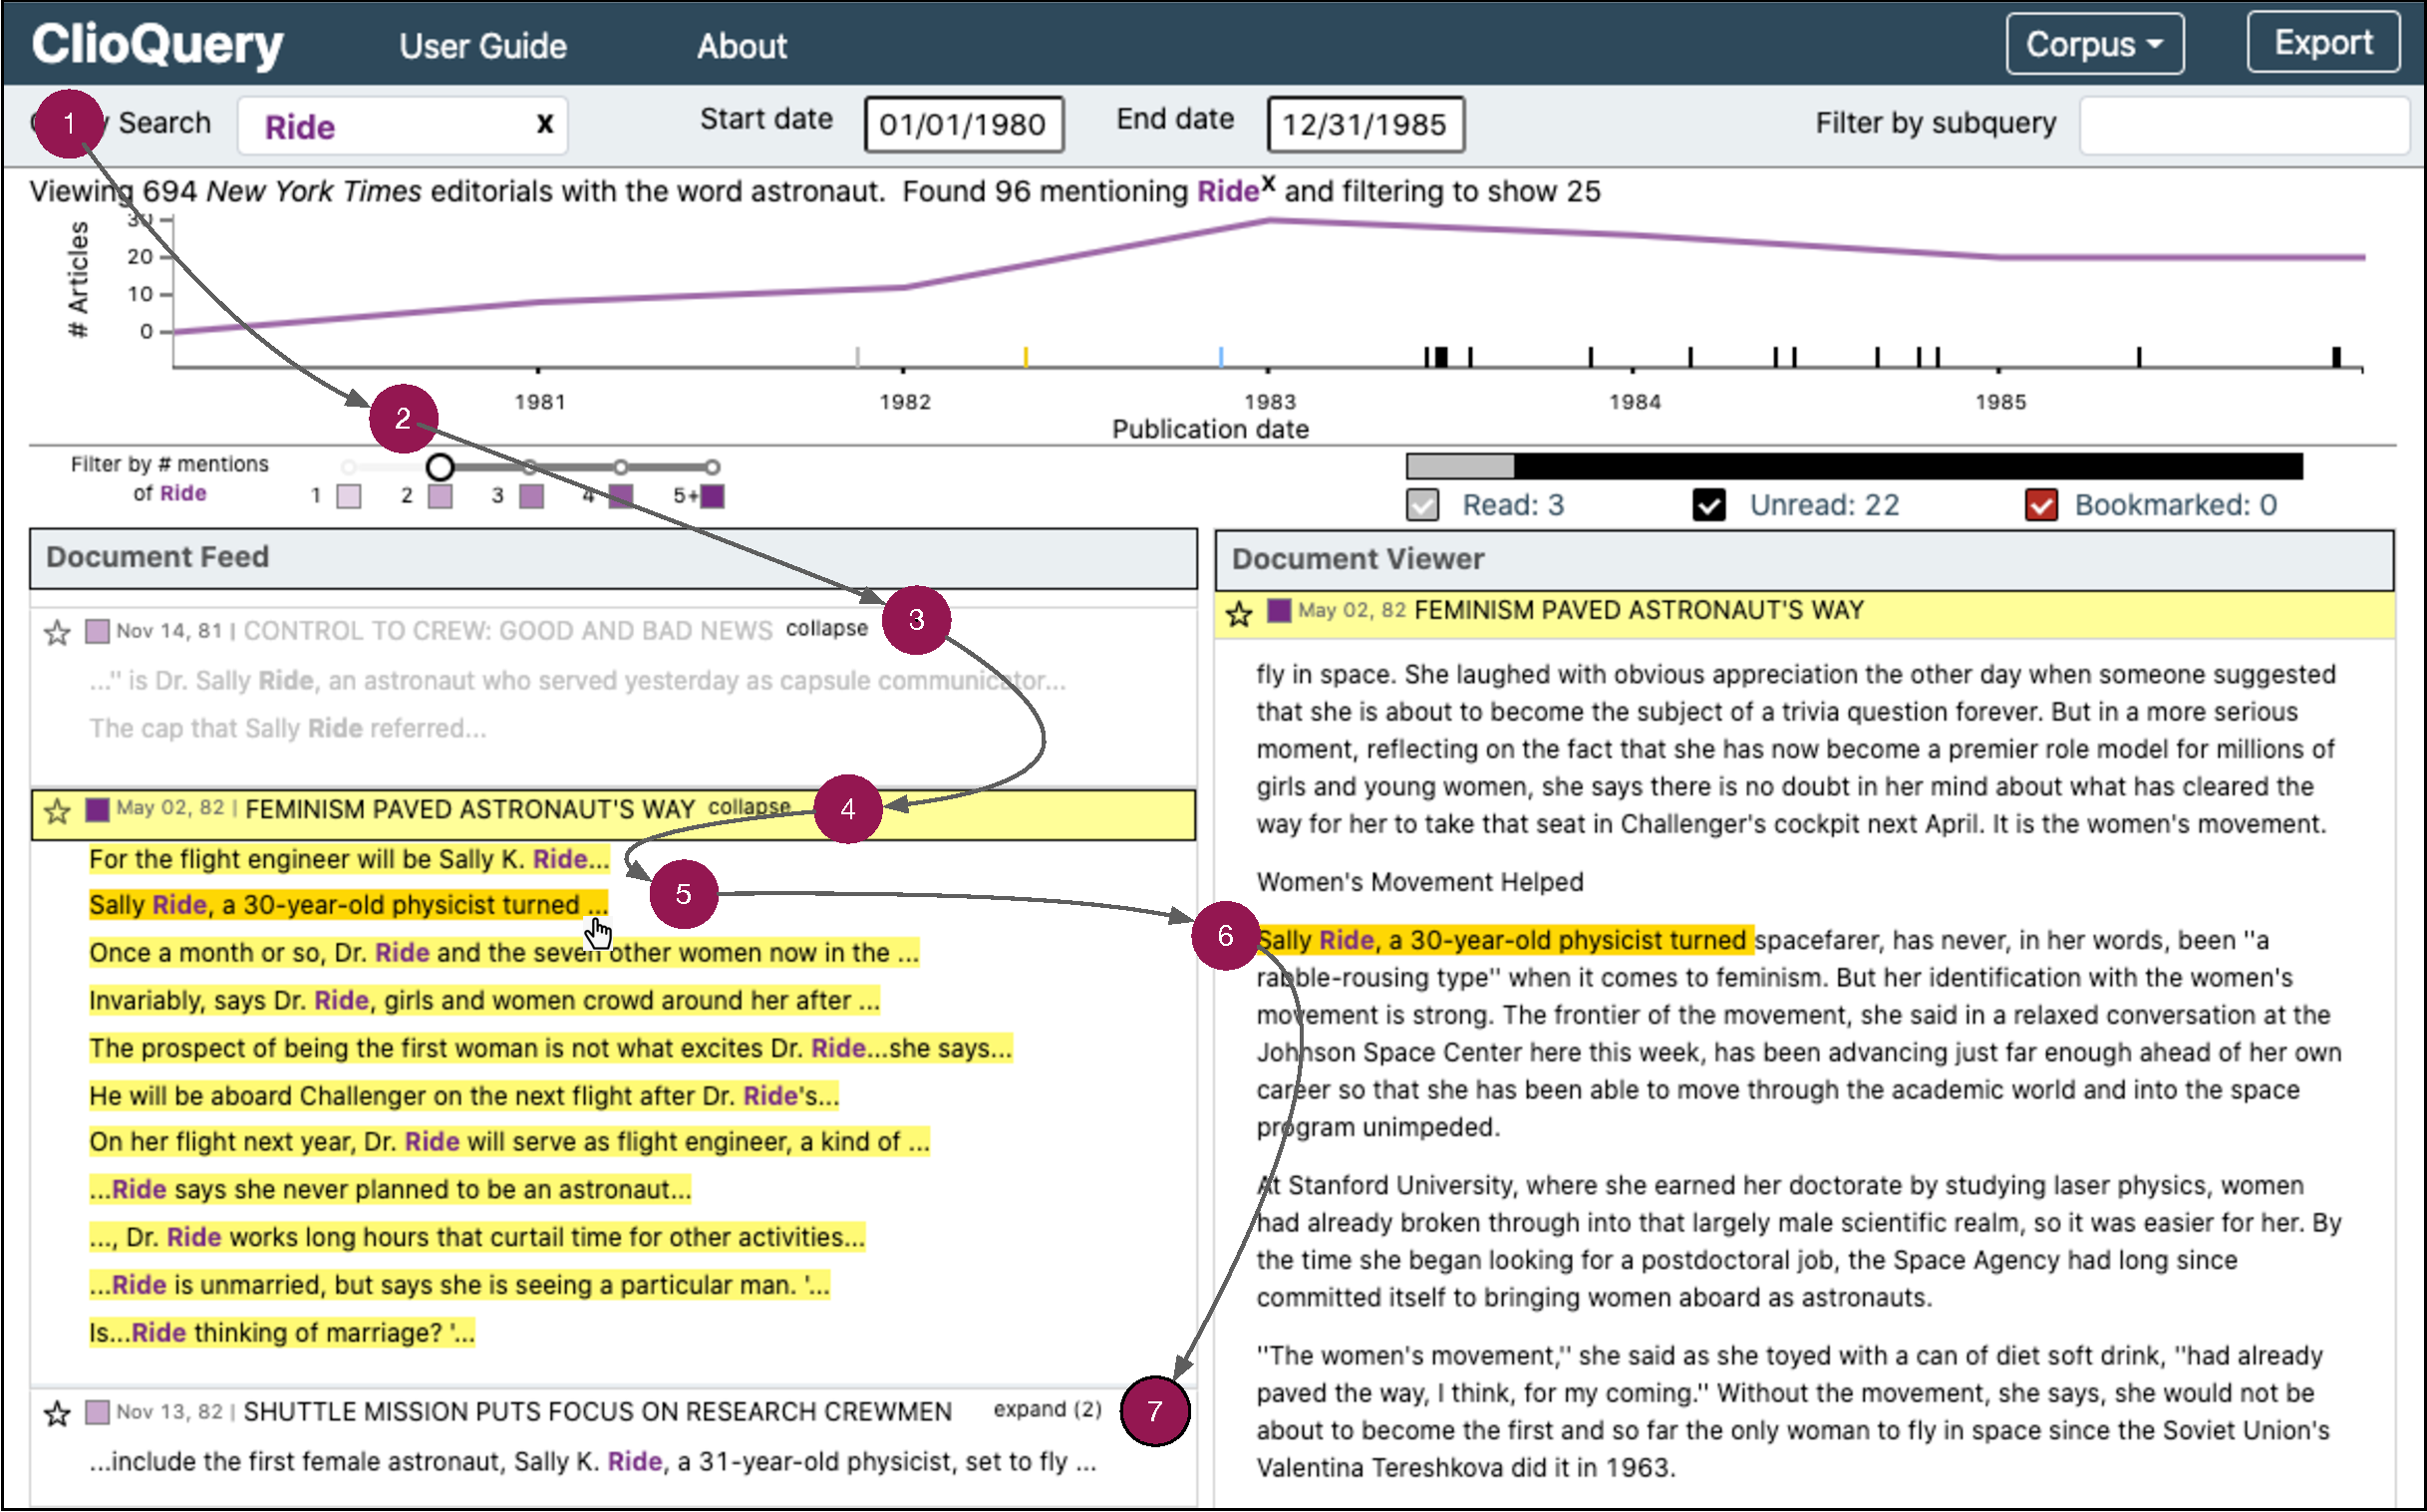
\includegraphics[width=.683\linewidth]{figures/workflow_fig/open_locate_loop_CC.pdf}  
 \subcaption{
% \footnotesize %  uncomment for thesis
 A user (1) searches for ``Ride'' using \ours~and (2) sets the filter-by-count slider to limit results to stories with at least two mentions of ``Ride''. The user then clicks the expand/collapse button on two news stories (3 and 4) to review all mentions of Ride from each story in the Document Feed. They then (5) click one shortened sentence mentioning ``Ride'' (6) to read it within the context of the full original document in the linked Document Viewer, with help from automatic in-text highlighting. The user then prepares to (7) click expand to review additional mentions of Ride in the next story.}\label{f:field_study_2}
\end{subfigure}
%In this figure, history tracking is disabled; articles the user has already read would normally be shown in grey.
\caption[A workflow with \ours~and a \Baselongname~tool]{
% \footnotesize % uncomment for thesis
Reviewing mentions of U.S.\ astronaut Sally Ride in~\textit{The New York Times}, using \ours~(bottom) and a \Baselongname~tool (top). 
This particular example comes from our field study (Section \ref{s:fieldstudy}), where one historian commented on the advantages of the \ours~interface over a baseline \Baselongname~system.
\textit{ ``What can I do here [with \ours] that I can't do there [with \textit{New York Times} search]?"} she said. 
\textit{``It's exploring this left-hand Document Feed.''}
Where \ours~facilitates quick and comprehensive review of all query mentions, the \Baselongname~tool requires the user to read unnecessary passages and context switch across documents.
}\label{f:field_study_loop}
\end{figure}

